\begin{frame}
	\frametitle{La aplicación \BulletPoint{}}
	\begin{columns}
		\begin{column}{0.6\textwidth}
			\block{Localización de transporte público, horarios e información de la parada}
			\begin{itemize}
				\item Objetivo.
				\item Despliegue.
				\item Funcionamiento.
				\item Dificultades.
				\item Ampliación.
			\end{itemize}
			\endblock{}
		\end{column}
		\begin{column}{0.4\textwidth}
			\vfill 
			\begin{center}
				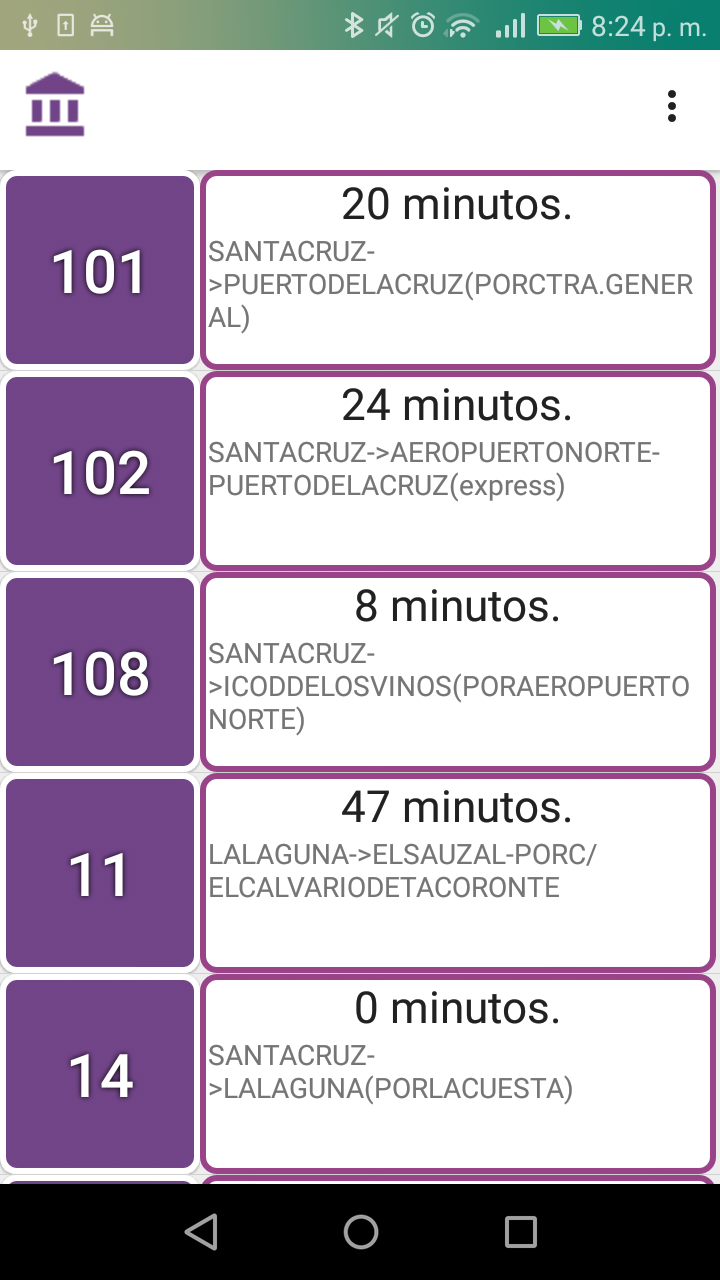
\includegraphics[width=0.8\linewidth]{Images/App/Autobuses}
			\end{center}
		\end{column}
	\end{columns}
\end{frame}

%--------------------------------------------------------------------

\begin{frame}
	\frametitle{Asociación de MAC a identificador de parada}
	\lstinputlisting{Code/BeaconBusStop.java}
\end{frame}

%--------------------------------------------------------------------

\begin{frame}
	\frametitle{Petición API TITSA}
	\lstinputlisting{Code/HttpClientTitsaJsoup.java}
\end{frame}

%--------------------------------------------------------------------

\begin{frame}
	\frametitle{La aplicación \BulletPoint{}}
	\begin{columns}
		\begin{column}{0.6\textwidth}
			\block{Gestión de eventos e información}
			\begin{itemize}
				\item Objetivo.
				\item Despliegue.
				\item Funcionamiento.
				\item Dificultades.
				\item Ampliación.
			\end{itemize}
			\endblock{}
		\end{column}
		\begin{column}{0.4\textwidth}
			\vfill 
			\begin{center}
				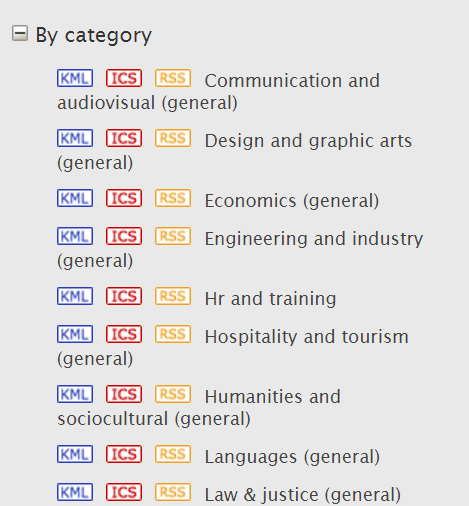
\includegraphics[width=0.7\linewidth]{Images/eventsRss}
			\end{center}
		\end{column}
	\end{columns}
\end{frame}

%--------------------------------------------------------------------

\begin{frame}
	\frametitle{Asociación de MAC a enlace RSS}
	\lstinputlisting{Code/RssBeaconInfo.java}
\end{frame}

%--------------------------------------------------------------------

\begin{frame}
	\frametitle{La aplicación \BulletPoint{}}
		\block{Control de asistencia}
		\begin{itemize}
			\item Objetivo.
			\item Despliegue.
			\item Funcionamiento.
			\item Dificultades.
			\item Ampliación.
		\end{itemize}
		\endblock{}
\end{frame}

%--------------------------------------------------------------------

\begin{frame}
	\frametitle{Preferencias de usuario}
	\lstinputlisting{Code/preferences.xml}
\end{frame}

%--------------------------------------------------------------------

\begin{frame}
	\frametitle{Comprobando la localización en el área}
	\lstinputlisting{Code/scanAtt.java}
\end{frame}

%--------------------------------------------------------------------

\begin{frame}
	\frametitle{La aplicación \BulletPoint{}}
		\block{Guía a través del campus de la universidad}
		\begin{itemize}
			\item Objetivo.
			\item Despliegue.
			\item Funcionamiento.
			\item Dificultades.
			\item Ampliación.
		\end{itemize}
		\endblock{}
\end{frame}

%--------------------------------------------------------------------

\begin{frame}
	\frametitle{Mostrar la posición del usuario en la imagen}
	\lstinputlisting{Code/threeMainFunctionTrilaterate.java}
\end{frame}

\begin{frame}
	\frametitle{La aplicación \BulletPoint{}}
	\begin{columns}
		\begin{column}{0.6\textwidth}
			\block{Acceso al parking}
			\begin{itemize}
				\item Objetivo.
				\item Despliegue.
				\item Funcionamiento.
				\item Dificultades.
				\item Ampliación.
			\end{itemize}
			\endblock{}
		\end{column}
		\begin{column}{0.4\textwidth}
			\vfill 
			\begin{center}
				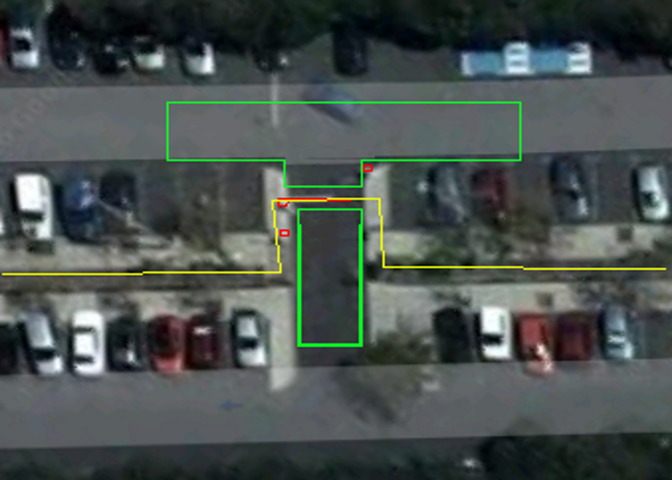
\includegraphics[width=0.9\linewidth]{Images/parking}
			\end{center}
		\end{column}
	\end{columns}
\end{frame}

%--------------------------------------------------------------------

\begin{frame}
	\frametitle{La aplicación \BulletPoint{}}
		Vídeo demostrativo de la aplicación \BulletPoint{}
\end{frame}